The proposed solution is based on the \emph{Scatter-Search} meta-heuristic,
and the implemented procedure is described in Algorithm \ref{alg:1}.

\begin{scriptsize}
\begin{algorithm}[h!t]
    \begin{algorithmic}
        \STATE solution\_generation()
        \STATE solution\_improvement()
        \STATE refset\_build()
        \STATE save\_the\_best\_solution()
        \REPEAT
            \WHILE {$\text{New solutions in RefSet}$}
                \STATE solution\_combination()
                \STATE solution\_improvement()
                \STATE refSet\_modification()
            \ENDWHILE
            \STATE save\_the\_best\_solution()
            \STATE refset\_rebuild()
        \UNTIL {iteration $<$ Max\_Iteration}
    \end{algorithmic}
    \caption{Scatter Search Procedure}
    \label{alg:1}
\end{algorithm}
\end{scriptsize}

Some fundamental details of each procedure,
is explained below:

\begin{itemize}
    \item $solution\_generation()$

        The solutions are generated considering an ordered sequence
        of the box identifiers, which is used as starting point.
        Each solution, use the starting point and perform a modification in the identifiers order \emph{randomly},
        to generate the $popsize$ solutions.

    \item $solution\_improvement()$
        Considering $N$ as the total amount of boxes,
        a \emph{swap} is performed $N/2$ times between two elements of the solution,
        the process is explained in \ref{fig:swap}.

        \begin{figure}[h!t]
            \centering
            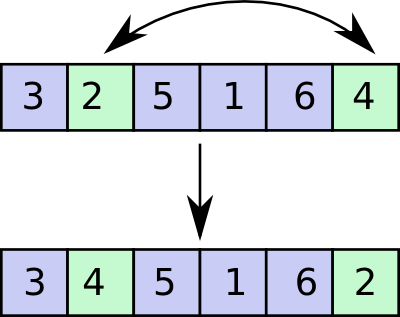
\includegraphics[width=0.3\textwidth]{img/ia-swap}
            \caption{Swap movement to improve solutions example.}
            \label{fig:swap}
        \end{figure}

    \item $refset\_build()$

        The $RefSet$ is constructed considering the $b$ best solutions,
        from the main solutions set.

    \item $save\_the\_best\_solution()$

        The $RefSet$ set is sorted, and the best solution is saved.

    \item $solution\_combination()$

        To combine the solutions, is proposed a Particle Matching Crossover (PMX),
        which consist in the selection of a sub-sequence position from solution,
        and the considering two solutions, the elements contained in the
        previous sub-sequence position are exchanged for each other.
        And example of PMX is described in \ref{fig:pmx}.

        \begin{figure}[h!t]
            \centering
            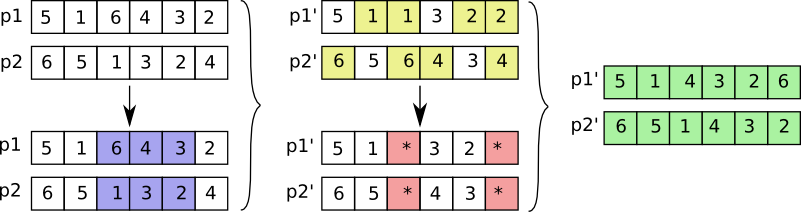
\includegraphics[width=0.8\textwidth]{img/ia-pmx}
            \caption{Partial Matching Crossover (PMX) example.}
            \label{fig:pmx}
        \end{figure}

    \item $refSet\_modification()$

        The $RefSet$ is modified following the next procedure:
        Select the $b$ best solutions between the union of the new
        $b(b-1)/2$ generated solutions in the inner-loop and the $RefSet$ solutions.

    \item $refset\_rebuild()$

        The rebuild is performed removing the $b/2$ worst solutions,
        and a new entire population of solutions are generated
        using the same mechanism of the algorithm first phase (before the outer-loop),
        but, the improvement is a different approach, using the \emph{shift} instead
        the previous \emph{swap}.
        The \emph{shift} \ref{fig:shift} is performed N times to the left,
        considering all the possible new sub-solutions for each solution,
        and the final used candidates are only the sub-solutions which their fitness
        is more distant from the previous one.
        Considering this new set of solutions, the worst solution are selected,
        because they are the more diverse solutions in comparison to the $RefSet$.
        Finally the selected solutions in both steps produces the new $RefSet$.

        \begin{figure}[h!t]
            \centering
            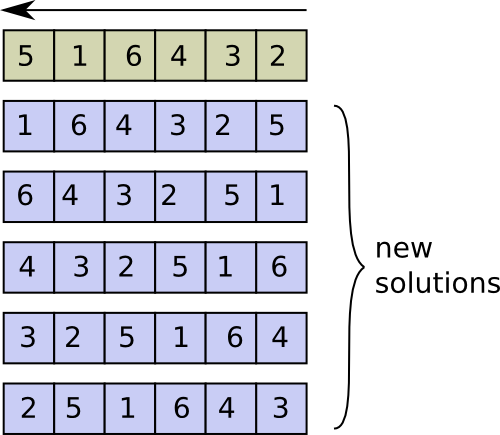
\includegraphics[width=0.5\textwidth]{img/ia-shift}
            \caption{Shift example.}
            \label{fig:shift}
        \end{figure}
\end{itemize}
